\section{Table Segmentation}

The following assumptions were made for the segmentation of the table:
\begin{itemize}
    \item the table is of uniform color and it is a prevalent part of the image;
    \item the table is centered (or close to being centered) in the image.
\end{itemize}

\noindent
The reason for these is going to be evident when the full algorithm for
the table segmentation is explained. \par
The first thing that had to be found was a rough segmentation of the table.
Finding the lines with only the Canny-transform of the full image was 
problematic, as the strongest lines in the image do not correspond to only the table
fabric, but also the table itself and other things in the image.
The initial approach was to use Otsu's thresholding. Since the table is of uniform
color, it was assumed that the table would have been thresholded the same
way throughout. Althought, this proved unfruitful because the obtained segmentation was too rough (Figure \ref{fig:otsutable}).
The second approach involved K-means clustering with Kmeans++ initialization, in particular exploiting the
adaptability of the algorithm to the use of spatial features to improve
the segmentation, as we assumed the table being a continuous entity. Out of the K clusters obtained, the most centered one was picked as shown in figure \ref{fig:kmeanstabol}. \par
The segmentation obtained was fairly precise but contained multiple disconnected
components. However, we can assume the table being the biggest one and pick it. Additionally,
before doing this, the morphological operation \textit{Opening} is applied in order to remove weakly connected objects.
The K parameter was empirically chosen as 3, since 2 lead to undersegmentation of the image and 4 to oversegmentation.
The resulting segmentation is precise in most cases, but given the nature of Kmeans, on some
images the algorithm fails because it clusterizes some unrelated parts of the table with the fabric, due,
for example, to lighting effects.
For this reason further processing was required: given the obtained rough mask of
the table, we now obtain the mean color of the image in the pixels where the mask is non-zero.
After this, we use a color thresholding by distance as shown in figure \ref{fig:colorsegtabol} from the mean and the same way we 
did before to obtain the largest connected component. Thresholding on the hue channel
was the most robust option (instead of using the distance between BGR colors). In particular, a low distance of $5$ was chosen, but different values close to $5$ showed similar results.\par
After having obtained this result, the morphological operation \textit{Close} was applied in order to remove some noise from the mask,
like balls and other objects. Afterwards the \textit{Hough Transform} algorithm is used to find the lines, 
with a threshold in order to remove similar ones.
The vertices of the table were found using the equations from \href{https://en.wikipedia.org/wiki/Line\%E2\%80\%93line\_intersection}{wikipedia}.
It must noted that the last frame is used for this task, as most of the time it doesn't contain the player in the table since it's the end of
his turn.
The segmentation found is technically not precise since we count as part of table player, holes and billiard balls. The latter can be easily solved by simply removing the areas of the balls that are detected. 
As for the other two cases, they were ignored for a compromise on performance, as in some
cases the change in illumination is severe, causing some parts of the table to have extreme 
differences in color, for example in the internal parts of the table. This isse was solved through 
the \textit{Hough Transform}.
It should also be considered that the morphological operations used to isolate the connected component of the table, also worsen
the general table outlines. For this reason the output of the line detection is preferred, as it yields
more consistent and stable results as shown in figure \ref{fig:finalsegtabol}.

\begin{figure}[h]
    \centering
    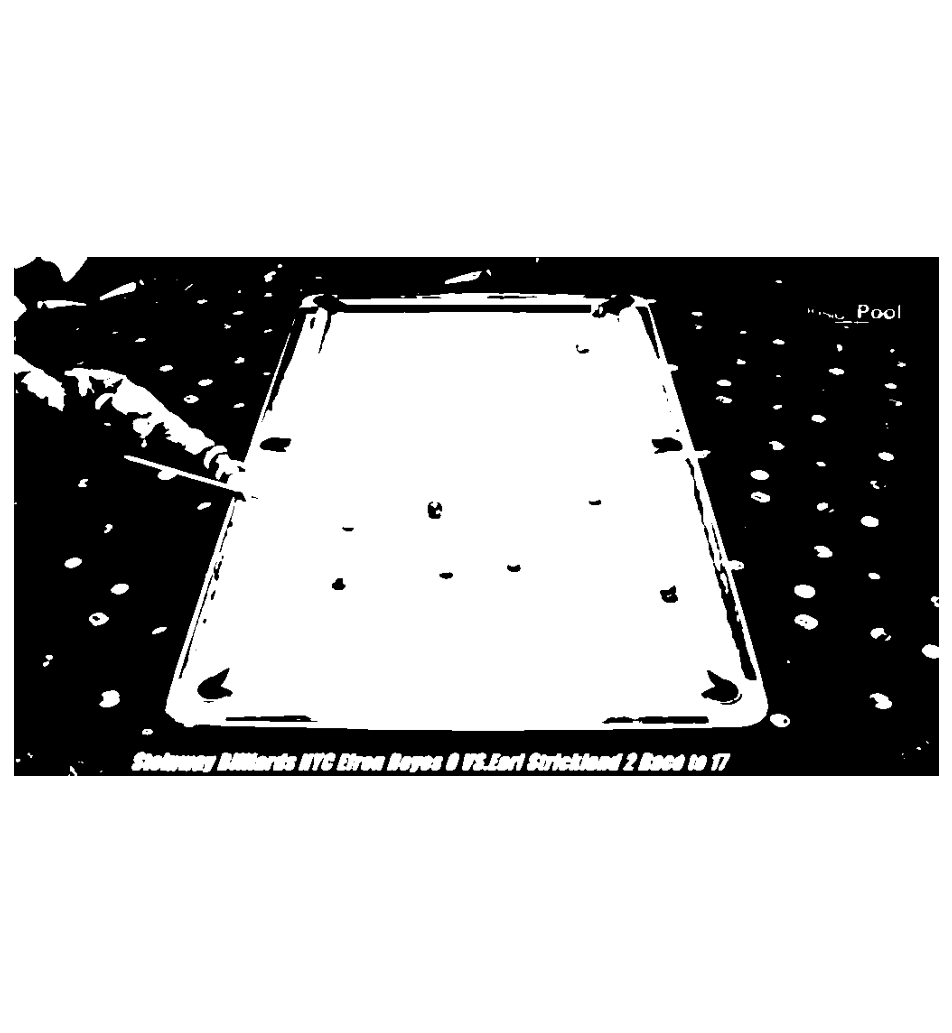
\includegraphics[width=0.4\textwidth]{./imgs/otsu_table.png}
    \caption{Example of Otsu Segmentation applied to game4\_clip2}
    \label{fig:otsutable}
\end{figure}

\begin{figure}
    \centering
    \begin{subfigure}[b]{0.75\textwidth}
        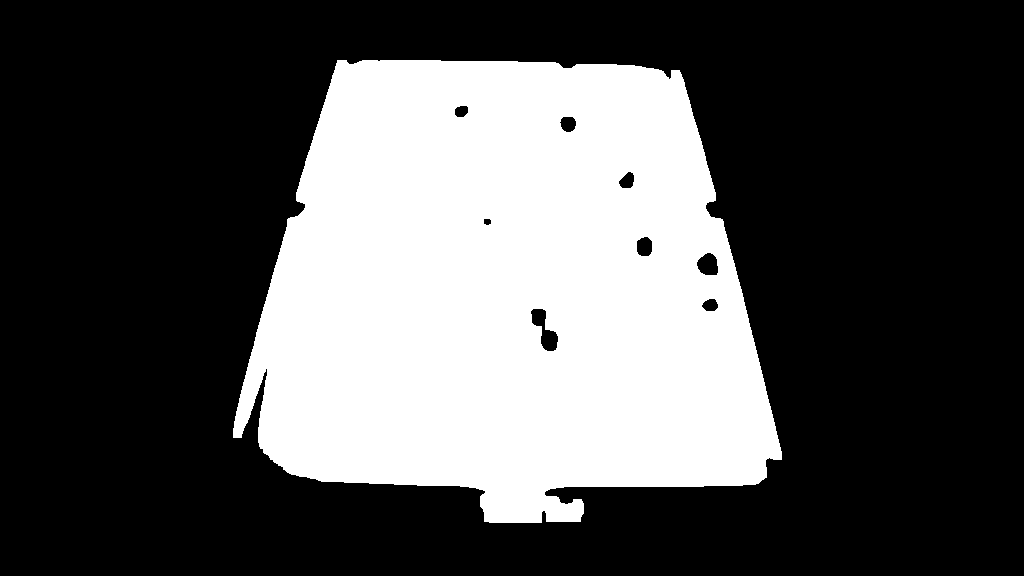
\includegraphics[width=\textwidth]{./imgs/kmeans_cluster.png}
        \caption{Initial Kmeans clustering result applied to game4\_clip2}
        \label{fig:kmeanstabol}
    \end{subfigure}
    \\
    \begin{subfigure}[b]{0.75\textwidth}
        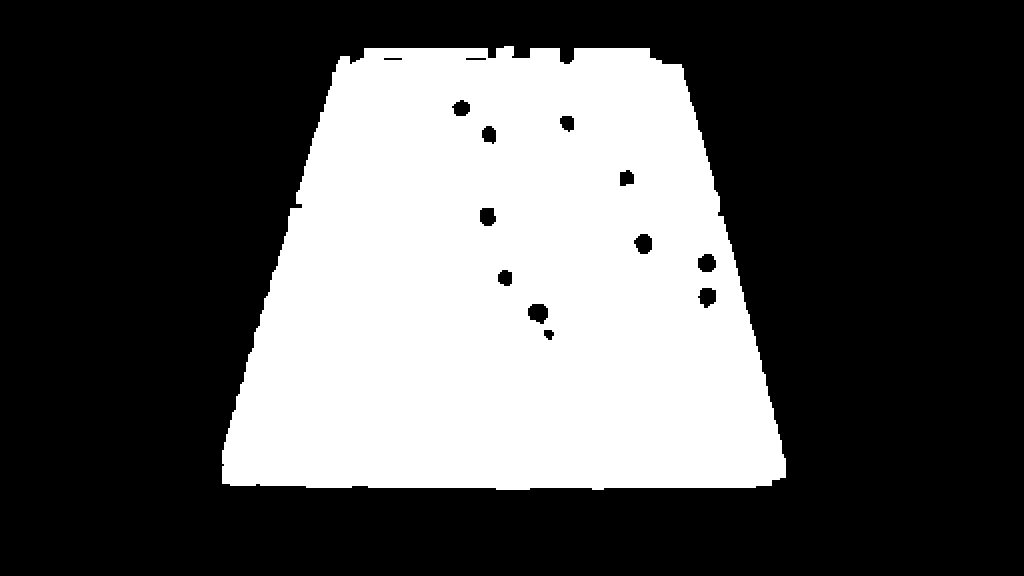
\includegraphics[width=\textwidth]{./imgs/color_cluster.png}
        \caption{Color clustering result}
        \label{fig:colorsegtabol}
    \end{subfigure}
    \\
    \begin{subfigure}[b]{0.75\textwidth}
        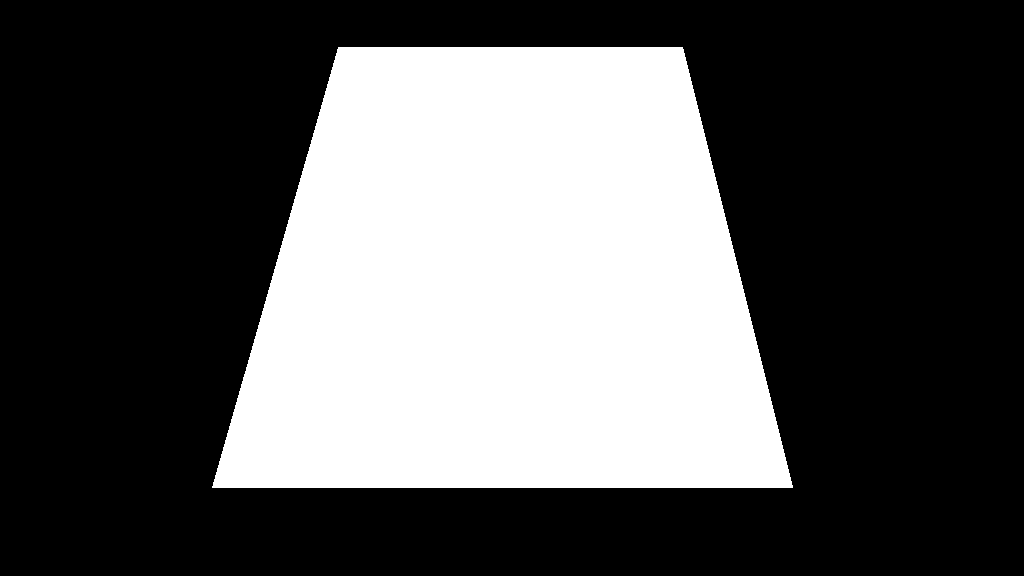
\includegraphics[width=\textwidth]{./imgs/maskfill.png}
        \caption{Mask obtained from filling the area contained in the lines found}
        \label{fig:finalsegtabol}
    \end{subfigure}
    \caption{Stages of the segmentation applied to game4\_clip2}
    \vspace{30pt}
\end{figure}
